% Created 2018-03-16 vie 12:49
\documentclass[letterpaper]{scrartcl}
\usepackage[utf8]{inputenc}
\usepackage[T1]{fontenc}
\usepackage{fixltx2e}
\usepackage{graphicx}
\usepackage{longtable}
\usepackage{float}
\usepackage{wrapfig}
\usepackage{rotating}
\usepackage[normalem]{ulem}
\usepackage{amsmath}
\usepackage{textcomp}
\usepackage{marvosym}
\usepackage{wasysym}
\usepackage{amssymb}
\usepackage{hyperref}
\tolerance=1000
\usepackage{khpreamble}
\usepackage{geometry}
\geometry{top=20mm, bottom=20mm, left=22mm, right=18mm}
\author{Kjartan Halvorsen}
\date{\today}
\title{State feedback with observer exercise}
\hypersetup{
  pdfkeywords={},
  pdfsubject={},
  pdfcreator={Emacs 24.5.1 (Org mode 8.2.10)}}
\begin{document}

\maketitle

\section*{Complete the block diagram}
\label{sec-1}
\begin{center}
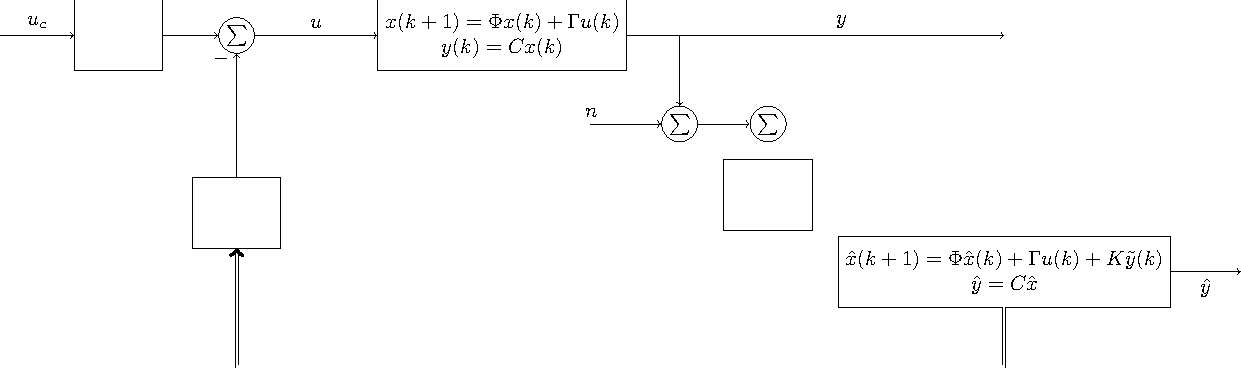
\includegraphics[width=\linewidth]{../figures/state-feedback-with-observer-incomplete}
\end{center}

The control law is \(u(k) = l_0u_c(k) - L\hat{x}(k)\). The feedback to the observer is \(K\tilde{y}(k) = K\big(y_m(k) - \hat{y}(k)\big) = K\big(y(k) + n(k) - C\hat{x}(k)\big) \) 


\section*{Complete the augmented state-space model}
\label{sec-2}

\begin{align*}
\bbm x(k+1)\\\hat{x}(k+1) \ebm &= \bbm & & & & & & & &&& & & &\\ &&& & & & & & & & & & &\ebm \bbm x(k)\\\hat{x}(k)\ebm + \bbm &&&\\&&&\\&&&\\&&& \ebm u_c(k) + \bbm &&&\\&&&\\&&&\\&&& \ebm n(k)\\
y(k) &= \bbm &&&&&& \ebm \bbm x(k)\\\hat{x}(k)\ebm
\end{align*}

\newpage

\section*{Control of a tank model}
\label{sec-3}
Consider the system of two tanks in the figure below. The input signal is the flow of water into the upper tank, and the output signal is the level of the second tank. 

\begin{minipage}{0.6\linewidth}
In continuous-time the system is described by the state space system
\begin{align*}
\frac{dx}{dt} &= \bbm -0.0197 & 0\\0.0178 & -0.0129 \ebm x + \bbm 0.0263\\0 \ebm u\\
y &= \bbm 0 & 1 \ebm x.
\end{align*}
With sampling period \(h=12\) we obtain the discrete-time system
\begin{align*}
x(kh+h) &= \bbm 0.790 & 0\\ 0.176 & 0.857 \ebm x(kh) + \bbm 0.281\\ 0.0296 \ebm u(kh)\\
y(kh) &= \bbm 0 & 1 \ebm x(kh).
\end{align*}
\end{minipage}
\begin{minipage}{0.4\linewidth}
 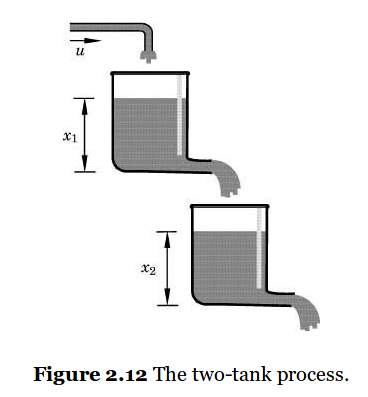
\includegraphics[width=\linewidth]{../figures/fig2-12-two-tank-system.png}
\end{minipage}


\begin{enumerate}
\item Determine an observer with poles that are twice as fast as the fastest mode of the plant.
\item Determine a state feedback gain \(L\) such that the closed-loop system has poles in \( 0.8 \pm 0.1\).
\end{enumerate}

\begin{center}
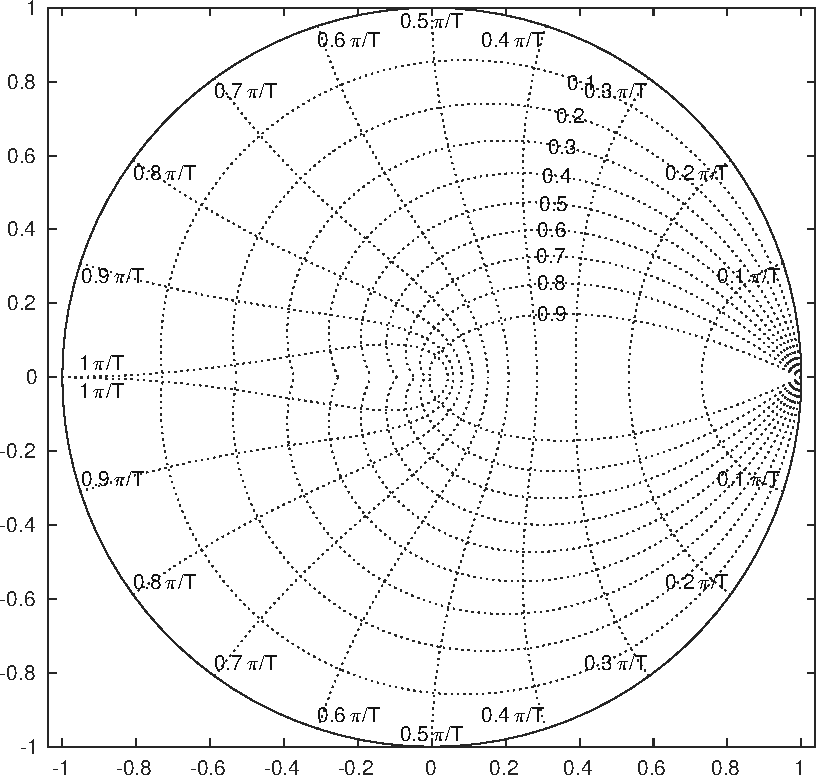
\includegraphics[width=0.45\linewidth]{../figures/zgrid-crop}
\end{center}

\newpage 

\section*{Implementing the controller}
\label{sec-4}
Complete the pseudo-code (matlab) below for the implementation of the controller
\begin{verbatim}
% The plant model
n = 2;
h = 12; 
Phi = [0.79 0; 0.176 0.857]; 
Gamma = [0.281; 0.0296];
C = [0 1];

% The controller and observer gains

L = 

K = 

% Initialize variables
u = 0; xhat = [0; 0];
% Run the controller 
while run_controller() % The function run_controller will return 0 if the controller should stop
   y = get_output();  % Returns the sampled output signal from the plant

   % Update the observer

   xhat = 

   % Compute the control signal

   u = 

   % Send the control signal to the plant
   write_control_signal(u);
   % Wait until next sampling instant
   sleep(h);
end
\end{verbatim}
% Emacs 24.5.1 (Org mode 8.2.10)
\end{document}